%% ECON 282E -- Session 7, Deck B1: The Growth Model via Euler Residuals
%% Sources: AI-ECON Lec04_T1_Motivation_Growth.tex, carried WHOLE (31 frames;
%% its "Appendix: Dynamic Macro Foundations" is a Solow-to-Bellman refresher
%% that S01_B1-B2 already cover, so it is not taught here);
%% AI-ECON Lec04_T3_Euler_PyTorch.tex, carried WHOLE (21 frames);
%% Quant_Macro Lec.9 frames 115-121 -- "Formulating the Euler Equation as a
%% Learning Problem", "Comparison with Collocation or Galerkin", "Connection to
%% Galerkin and Weighted Residual Methods" -- deferred to S7 by 5.B1 and
%% rewritten here with Fernandez-Villaverde & Guerron-Quintana cited;
%% Quant_Macro Lec.6 "Euler Equation Based + ML" and "Pytorch Implementation";
%% Feng & Miao, "AI for Economists" (Book1), ch.10 "From equilibrium conditions
%% to a loss function".
%% Numbers from tools/figures/s07_numbers.json, keys "worked_nn_growth",
%% "five_methods", "param_count"; the first four rows of the methods table are
%% READ from s05_numbers.json key "three_methods", never recomputed.

%% ECON 282E -- Foundations of Macroeconomics (UC Riverside, Fall 2026)
%% Shared Beamer preamble for every deck in slides/S01 ... slides/S10.
%%
%% Usage (a deck lives in slides/S0X/ and is compiled from that folder):
%%   %% ECON 282E -- Foundations of Macroeconomics (UC Riverside, Fall 2026)
%% Shared Beamer preamble for every deck in slides/S01 ... slides/S10.
%%
%% Usage (a deck lives in slides/S0X/ and is compiled from that folder):
%%   %% ECON 282E -- Foundations of Macroeconomics (UC Riverside, Fall 2026)
%% Shared Beamer preamble for every deck in slides/S01 ... slides/S10.
%%
%% Usage (a deck lives in slides/S0X/ and is compiled from that folder):
%%   \input{../preamble/course_preamble.tex}
%%   \decktitle{1}{A1}{Who I Am \& Why This Course}{September 24, 2026}
%%   \begin{document}
%%   \makedecktitle
%%   ...
%%
%% Adapted from Courses/AI-ECON-2026/source/shared_preamble.tex (Metropolis theme,
%% concept/caution/example/takeaway boxes, \sectiondivider). Changes for this course:
%%   * course title block (\decktitle / \makedecktitle) instead of \makebeamertitle
%%   * \zh{...} typesets Chinese (book titles) under pdflatex via CJKutf8
%%   * researchbox for the "Research in the wild" frames
%%   * section pages off; TikZ libraries and the course map loaded here
%% Build with pdflatex only (two passes); tools/build_slides.py does this for you.

\documentclass[10pt,english,aspectratio=169]{beamer}

\usepackage[T1]{fontenc}
\usepackage{textcomp}
\usepackage[utf8]{inputenc}
\usepackage{babel}
\usepackage{CJKutf8}

\usepackage{amsmath, amssymb, amsthm, graphicx}
\usepackage{booktabs, multirow, tabularx}
\usepackage{tikz}
\usetikzlibrary{positioning,arrows.meta,shapes,calc,fit,backgrounds}
\usepackage{pgfplots}
\pgfplotsset{compat=1.16}
\usepackage[most]{tcolorbox}
\tcbuselibrary{skins, breakable}
\usepackage{listings}
\usepackage{xcolor}

\lstset{
  basicstyle=\ttfamily\small,
  keywordstyle=\color{blue!80!black}\bfseries,
  commentstyle=\color{green!50!black}\itshape,
  stringstyle=\color{orange!80!black},
  backgroundcolor=\color{gray!8},
  frame=single,
  rulecolor=\color{gray!40},
  breaklines=true,
  showstringspaces=false,
  numbers=none,
}

\usetheme{metropolis}
\usefonttheme{professionalfonts}
\metroset{sectionpage=none}

\definecolor{LightGray}{RGB}{230,230,230}
\definecolor{RedTitle}{RGB}{0,0,200}
\definecolor{VeryLightGray}{RGB}{245,245,245}
\definecolor{DarkText}{RGB}{0,0,0}
\definecolor{UCRBlue}{RGB}{0,45,106}
\definecolor{UCRGold}{RGB}{241,171,0}

% Stage colours of the course arc (used by the course map and elsewhere)
\colorlet{StageTrunk}{blue!12}
\colorlet{StageBranch}{cyan!14}
\colorlet{StageMachine}{gray!18}
\colorlet{StageWall}{red!14}
\colorlet{StageTools}{orange!20}
\colorlet{StageData}{green!16}
\colorlet{StageAgents}{violet!14}

\hypersetup{bookmarks=false,breaklinks=true,pdfborder={0 0 0},colorlinks=true,
  linkcolor=DarkText,urlcolor=RedTitle}

\setbeamercolor{background canvas}{bg=white}
\setbeamercolor{title}{fg=RedTitle}
\setbeamercolor{frametitle}{bg=VeryLightGray,fg=DarkText}
\setbeamercolor{normal text}{fg=DarkText}
\setbeamercolor{alerted text}{fg=RedTitle}
\setbeamersize{text margin left=5mm, text margin right=5mm}
\addtobeamertemplate{frametitle}{}{\vspace{-0.5em}}

\setbeamertemplate{navigation symbols}{}
\setbeamertemplate{footline}{%
  \hspace{5mm}{\usebeamerfont{page number in head/foot}\color{black!45}%
  ECON 282E \,$\cdot$\, \insertshortdeck}\hfill%
  \usebeamercolor[fg]{page number in head/foot}%
  \usebeamerfont{page number in head/foot}%
  \insertframenumber\,/\,\inserttotalframenumber\kern1em\vskip2pt%
}

% ---------------------------------------------------------------------------
% Chinese text under pdflatex (book titles etc.)
\newcommand{\zh}[1]{\begin{CJK*}{UTF8}{gbsn}#1\end{CJK*}}

% ---------------------------------------------------------------------------
% Deck title block
%   \decktitle{session}{deck id}{title}{date}
\newcommand{\insertshortdeck}{}
\newcommand{\decksession}{}
\newcommand{\deckid}{}
\newcommand{\decktitletext}{}
\newcommand{\deckdate}{}
\newcommand{\decktitle}[4]{%
  \renewcommand{\decksession}{#1}%
  \renewcommand{\deckid}{#2}%
  \renewcommand{\decktitletext}{#3}%
  \renewcommand{\deckdate}{#4}%
  \renewcommand{\insertshortdeck}{Session #1 \,$\cdot$\, Deck #1.#2}%
  \title{#3}%
  \author{Zhigang Feng}%
  \date{#4}%
}
\newcommand{\makedecktitle}{%
  \begin{frame}[plain,noframenumbering]
    \begin{tikzpicture}[remember picture,overlay]
      \fill[UCRBlue] (current page.north west) rectangle ([yshift=-0.55cm]current page.north east);
      \fill[UCRGold] ([yshift=-0.55cm]current page.north west) rectangle ([yshift=-0.62cm]current page.north east);
      \node[anchor=west, text=white, font=\small\bfseries] at ([xshift=5mm,yshift=-0.275cm]current page.north west)
        {ECON 282E \,$\cdot$\, Foundations of Macroeconomics};
      \node[anchor=east, text=white, font=\small] at ([xshift=-5mm,yshift=-0.275cm]current page.north east)
        {UC Riverside \,$\cdot$\, Fall 2026};
    \end{tikzpicture}
    \vspace*{1.1cm}
    {\usebeamerfont{title}\color{black!55}\large Session \decksession\ \,$\cdot$\, Deck \decksession.\deckid\par}
    \vspace{0.25cm}
    {\usebeamerfont{title}\color{RedTitle}\LARGE\bfseries \decktitletext\par}
    \vspace{0.7cm}
    {\large Zhigang Feng\par}
    \vspace{0.15cm}
    {\color{black!65}\deckdate\par}
    \vfill
    {\footnotesize\itshape\color{black!55}Build it on paper $\;\to\;$ solve it on the machine $\;\to\;$ push it to the frontier with AI\par}
  \end{frame}}

% ---------------------------------------------------------------------------
% Section divider (plain frame, not counted)
\newcommand{\sectiondivider}[2]{%
\begin{frame}[plain,noframenumbering]
\begin{center}
\vfill
{\Large\textbf{#1}\par}
\vspace{0.35cm}
{\normalsize #2\par}
\vfill
\end{center}
\end{frame}
}

% ---------------------------------------------------------------------------
% Boxes
\newtcolorbox{conceptbox}[1][]{colback=blue!3, colframe=RedTitle!55, boxrule=0.35mm,
  arc=1mm, left=2mm, right=2mm, top=1mm, bottom=1mm, #1}
\newtcolorbox{cautionbox}[1][]{colback=red!3, colframe=red!50!black, boxrule=0.35mm,
  arc=1mm, left=2mm, right=2mm, top=1mm, bottom=1mm, #1}
\newtcolorbox{examplebox}[1][]{colback=green!3, colframe=green!45!black, boxrule=0.35mm,
  arc=1mm, left=2mm, right=2mm, top=1mm, bottom=1mm, #1}
\newtcolorbox{takeawaybox}[1][]{colback=VeryLightGray, colframe=RedTitle!55, boxrule=0.35mm,
  arc=1mm, left=2mm, right=2mm, top=1mm, bottom=1mm, #1}
\newtcolorbox{researchbox}[1][]{enhanced, colback=violet!4, colframe=violet!60!black,
  boxrule=0.35mm, arc=1mm, left=2mm, right=2mm, top=1mm, bottom=1mm,
  fonttitle=\bfseries\small, title={Research in the wild}, #1}

\newcommand{\compacttables}{\renewcommand{\arraystretch}{1.15}}
\newcommand{\src}[1]{{\tiny\color{black!55}#1}}

% ---------------------------------------------------------------------------
\input{../preamble/course_map.tex}

%%   \decktitle{1}{A1}{Who I Am \& Why This Course}{September 24, 2026}
%%   \begin{document}
%%   \makedecktitle
%%   ...
%%
%% Adapted from Courses/AI-ECON-2026/source/shared_preamble.tex (Metropolis theme,
%% concept/caution/example/takeaway boxes, \sectiondivider). Changes for this course:
%%   * course title block (\decktitle / \makedecktitle) instead of \makebeamertitle
%%   * \zh{...} typesets Chinese (book titles) under pdflatex via CJKutf8
%%   * researchbox for the "Research in the wild" frames
%%   * section pages off; TikZ libraries and the course map loaded here
%% Build with pdflatex only (two passes); tools/build_slides.py does this for you.

\documentclass[10pt,english,aspectratio=169]{beamer}

\usepackage[T1]{fontenc}
\usepackage{textcomp}
\usepackage[utf8]{inputenc}
\usepackage{babel}
\usepackage{CJKutf8}

\usepackage{amsmath, amssymb, amsthm, graphicx}
\usepackage{booktabs, multirow, tabularx}
\usepackage{tikz}
\usetikzlibrary{positioning,arrows.meta,shapes,calc,fit,backgrounds}
\usepackage{pgfplots}
\pgfplotsset{compat=1.16}
\usepackage[most]{tcolorbox}
\tcbuselibrary{skins, breakable}
\usepackage{listings}
\usepackage{xcolor}

\lstset{
  basicstyle=\ttfamily\small,
  keywordstyle=\color{blue!80!black}\bfseries,
  commentstyle=\color{green!50!black}\itshape,
  stringstyle=\color{orange!80!black},
  backgroundcolor=\color{gray!8},
  frame=single,
  rulecolor=\color{gray!40},
  breaklines=true,
  showstringspaces=false,
  numbers=none,
}

\usetheme{metropolis}
\usefonttheme{professionalfonts}
\metroset{sectionpage=none}

\definecolor{LightGray}{RGB}{230,230,230}
\definecolor{RedTitle}{RGB}{0,0,200}
\definecolor{VeryLightGray}{RGB}{245,245,245}
\definecolor{DarkText}{RGB}{0,0,0}
\definecolor{UCRBlue}{RGB}{0,45,106}
\definecolor{UCRGold}{RGB}{241,171,0}

% Stage colours of the course arc (used by the course map and elsewhere)
\colorlet{StageTrunk}{blue!12}
\colorlet{StageBranch}{cyan!14}
\colorlet{StageMachine}{gray!18}
\colorlet{StageWall}{red!14}
\colorlet{StageTools}{orange!20}
\colorlet{StageData}{green!16}
\colorlet{StageAgents}{violet!14}

\hypersetup{bookmarks=false,breaklinks=true,pdfborder={0 0 0},colorlinks=true,
  linkcolor=DarkText,urlcolor=RedTitle}

\setbeamercolor{background canvas}{bg=white}
\setbeamercolor{title}{fg=RedTitle}
\setbeamercolor{frametitle}{bg=VeryLightGray,fg=DarkText}
\setbeamercolor{normal text}{fg=DarkText}
\setbeamercolor{alerted text}{fg=RedTitle}
\setbeamersize{text margin left=5mm, text margin right=5mm}
\addtobeamertemplate{frametitle}{}{\vspace{-0.5em}}

\setbeamertemplate{navigation symbols}{}
\setbeamertemplate{footline}{%
  \hspace{5mm}{\usebeamerfont{page number in head/foot}\color{black!45}%
  ECON 282E \,$\cdot$\, \insertshortdeck}\hfill%
  \usebeamercolor[fg]{page number in head/foot}%
  \usebeamerfont{page number in head/foot}%
  \insertframenumber\,/\,\inserttotalframenumber\kern1em\vskip2pt%
}

% ---------------------------------------------------------------------------
% Chinese text under pdflatex (book titles etc.)
\newcommand{\zh}[1]{\begin{CJK*}{UTF8}{gbsn}#1\end{CJK*}}

% ---------------------------------------------------------------------------
% Deck title block
%   \decktitle{session}{deck id}{title}{date}
\newcommand{\insertshortdeck}{}
\newcommand{\decksession}{}
\newcommand{\deckid}{}
\newcommand{\decktitletext}{}
\newcommand{\deckdate}{}
\newcommand{\decktitle}[4]{%
  \renewcommand{\decksession}{#1}%
  \renewcommand{\deckid}{#2}%
  \renewcommand{\decktitletext}{#3}%
  \renewcommand{\deckdate}{#4}%
  \renewcommand{\insertshortdeck}{Session #1 \,$\cdot$\, Deck #1.#2}%
  \title{#3}%
  \author{Zhigang Feng}%
  \date{#4}%
}
\newcommand{\makedecktitle}{%
  \begin{frame}[plain,noframenumbering]
    \begin{tikzpicture}[remember picture,overlay]
      \fill[UCRBlue] (current page.north west) rectangle ([yshift=-0.55cm]current page.north east);
      \fill[UCRGold] ([yshift=-0.55cm]current page.north west) rectangle ([yshift=-0.62cm]current page.north east);
      \node[anchor=west, text=white, font=\small\bfseries] at ([xshift=5mm,yshift=-0.275cm]current page.north west)
        {ECON 282E \,$\cdot$\, Foundations of Macroeconomics};
      \node[anchor=east, text=white, font=\small] at ([xshift=-5mm,yshift=-0.275cm]current page.north east)
        {UC Riverside \,$\cdot$\, Fall 2026};
    \end{tikzpicture}
    \vspace*{1.1cm}
    {\usebeamerfont{title}\color{black!55}\large Session \decksession\ \,$\cdot$\, Deck \decksession.\deckid\par}
    \vspace{0.25cm}
    {\usebeamerfont{title}\color{RedTitle}\LARGE\bfseries \decktitletext\par}
    \vspace{0.7cm}
    {\large Zhigang Feng\par}
    \vspace{0.15cm}
    {\color{black!65}\deckdate\par}
    \vfill
    {\footnotesize\itshape\color{black!55}Build it on paper $\;\to\;$ solve it on the machine $\;\to\;$ push it to the frontier with AI\par}
  \end{frame}}

% ---------------------------------------------------------------------------
% Section divider (plain frame, not counted)
\newcommand{\sectiondivider}[2]{%
\begin{frame}[plain,noframenumbering]
\begin{center}
\vfill
{\Large\textbf{#1}\par}
\vspace{0.35cm}
{\normalsize #2\par}
\vfill
\end{center}
\end{frame}
}

% ---------------------------------------------------------------------------
% Boxes
\newtcolorbox{conceptbox}[1][]{colback=blue!3, colframe=RedTitle!55, boxrule=0.35mm,
  arc=1mm, left=2mm, right=2mm, top=1mm, bottom=1mm, #1}
\newtcolorbox{cautionbox}[1][]{colback=red!3, colframe=red!50!black, boxrule=0.35mm,
  arc=1mm, left=2mm, right=2mm, top=1mm, bottom=1mm, #1}
\newtcolorbox{examplebox}[1][]{colback=green!3, colframe=green!45!black, boxrule=0.35mm,
  arc=1mm, left=2mm, right=2mm, top=1mm, bottom=1mm, #1}
\newtcolorbox{takeawaybox}[1][]{colback=VeryLightGray, colframe=RedTitle!55, boxrule=0.35mm,
  arc=1mm, left=2mm, right=2mm, top=1mm, bottom=1mm, #1}
\newtcolorbox{researchbox}[1][]{enhanced, colback=violet!4, colframe=violet!60!black,
  boxrule=0.35mm, arc=1mm, left=2mm, right=2mm, top=1mm, bottom=1mm,
  fonttitle=\bfseries\small, title={Research in the wild}, #1}

\newcommand{\compacttables}{\renewcommand{\arraystretch}{1.15}}
\newcommand{\src}[1]{{\tiny\color{black!55}#1}}

% ---------------------------------------------------------------------------
%% Course map: the recurring "you are here" slide for ECON 282E.
%% Loaded by course_preamble.tex. Pattern follows AI-ECON-2026 lec01_map.tex, but the map
%% shows the whole ten-session course rather than one lecture.
%%
%%   \CourseMap{s}{label}   s = 1..10 highlights session s and prints "you are here: label"
%%                          (e.g. \CourseMap{1}{1.A2}); earlier sessions get a check mark.
%%   \CourseMap{0}{}        full overview, nothing highlighted.
%%
%% Note: TikZ option lists are comma-split before TeX conditionals run, so every \ifnum
%% below sits outside [...] option lists.

\newcommand{\CourseMap}[2]{%
\begin{center}
\begin{tikzpicture}[
    sess/.style={rectangle, rounded corners=2pt, draw=black!45, minimum width=1.34cm,
        minimum height=1.12cm, text width=1.26cm, align=center, inner sep=1pt},
    stage/.style={font=\tiny\bfseries, text=black!70},
]
  \foreach \i/\d/\t/\c in {%
      1/Sep 24/Intro \\ Growth/StageTrunk,
      2/Oct 1/HA $\cdot$ OLG \\ Policy/StageBranch,
      3/Oct 8/Num.\ DP \\ Python/StageMachine,
      4/Oct 15/Numerics \\ I/StageMachine,
      5/Oct 22/Numerics \\ II/StageMachine,
      6/Oct 29/The wall \\ \textbf{Midterm}/StageWall,
      7/Nov 5/ML \\ Deep nets/StageTools,
      8/Nov 12/RL \\ HA $+$ DL/StageTools,
      9/Nov 19/Text \\ LLMs/StageData,
      10/Dec 3/Agents \\ \textbf{Projects}/StageAgents} {
    \node[sess, fill=\c] (n\i) at ({1.46*(\i-1)}, 0)
      {{\scriptsize\bfseries S\i}\\[-1pt]{\tiny\color{black!60}\d}\\[1pt]{\tiny \t}};
    \ifnum\i<#1
      \node[font=\scriptsize, text=green!45!black] at ([xshift=-2.5mm,yshift=-2.2mm]n\i.north east) {$\checkmark$};
    \fi
    \ifnum\i=#1
      \draw[RedTitle, very thick, rounded corners=2pt]
        ([xshift=-0.6mm,yshift=-0.6mm]n\i.south west) rectangle ([xshift=0.6mm,yshift=0.6mm]n\i.north east);
      % keep the label inside the picture at both ends of the row
      \ifnum\i<3
        \node[font=\scriptsize\bfseries, text=RedTitle, anchor=south west] at ([yshift=1.2mm]n\i.north west)
          {$\blacktriangledown$\,you are here: #2};
      \else\ifnum\i>8
        \node[font=\scriptsize\bfseries, text=RedTitle, anchor=south east] at ([yshift=1.2mm]n\i.north east)
          {you are here: #2\,$\blacktriangledown$};
      \else
        \node[font=\scriptsize\bfseries, text=RedTitle, anchor=south] at ([yshift=1.2mm]n\i.north)
          {you are here: #2\,$\blacktriangledown$};
      \fi\fi
    \fi
  }
  % stage band under the sessions
  \foreach \a/\b/\lab/\c in {1/1/trunk/StageTrunk, 2/2/branches/StageBranch,
      3/5/the machine $\cdot$ classical methods/StageMachine, 6/6/the wall/StageWall,
      7/8/new tools/StageTools, 9/9/new data/StageData, 10/10/colleagues/StageAgents} {
    \fill[\c] ([yshift=-1.5mm]n\a.south west) rectangle ([yshift=-4.6mm]n\b.south east);
    \path ([yshift=-1.5mm]n\a.south west) -- ([yshift=-4.6mm]n\b.south east)
      node[midway, stage] {\lab};
  }
  \node[font=\footnotesize\itshape, text=black!70] at ([yshift=-9.5mm]$(n1.south)!0.5!(n10.south)$)
    {Build it on paper $\;\to\;$ solve it on the machine $\;\to\;$ push it to the frontier with AI};
\end{tikzpicture}
\end{center}
}


%%   \decktitle{1}{A1}{Who I Am \& Why This Course}{September 24, 2026}
%%   \begin{document}
%%   \makedecktitle
%%   ...
%%
%% Adapted from Courses/AI-ECON-2026/source/shared_preamble.tex (Metropolis theme,
%% concept/caution/example/takeaway boxes, \sectiondivider). Changes for this course:
%%   * course title block (\decktitle / \makedecktitle) instead of \makebeamertitle
%%   * \zh{...} typesets Chinese (book titles) under pdflatex via CJKutf8
%%   * researchbox for the "Research in the wild" frames
%%   * section pages off; TikZ libraries and the course map loaded here
%% Build with pdflatex only (two passes); tools/build_slides.py does this for you.

\documentclass[10pt,english,aspectratio=169]{beamer}

\usepackage[T1]{fontenc}
\usepackage{textcomp}
\usepackage[utf8]{inputenc}
\usepackage{babel}
\usepackage{CJKutf8}

\usepackage{amsmath, amssymb, amsthm, graphicx}
\usepackage{booktabs, multirow, tabularx}
\usepackage{tikz}
\usetikzlibrary{positioning,arrows.meta,shapes,calc,fit,backgrounds}
\usepackage{pgfplots}
\pgfplotsset{compat=1.16}
\usepackage[most]{tcolorbox}
\tcbuselibrary{skins, breakable}
\usepackage{listings}
\usepackage{xcolor}

\lstset{
  basicstyle=\ttfamily\small,
  keywordstyle=\color{blue!80!black}\bfseries,
  commentstyle=\color{green!50!black}\itshape,
  stringstyle=\color{orange!80!black},
  backgroundcolor=\color{gray!8},
  frame=single,
  rulecolor=\color{gray!40},
  breaklines=true,
  showstringspaces=false,
  numbers=none,
}

\usetheme{metropolis}
\usefonttheme{professionalfonts}
\metroset{sectionpage=none}

\definecolor{LightGray}{RGB}{230,230,230}
\definecolor{RedTitle}{RGB}{0,0,200}
\definecolor{VeryLightGray}{RGB}{245,245,245}
\definecolor{DarkText}{RGB}{0,0,0}
\definecolor{UCRBlue}{RGB}{0,45,106}
\definecolor{UCRGold}{RGB}{241,171,0}

% Stage colours of the course arc (used by the course map and elsewhere)
\colorlet{StageTrunk}{blue!12}
\colorlet{StageBranch}{cyan!14}
\colorlet{StageMachine}{gray!18}
\colorlet{StageWall}{red!14}
\colorlet{StageTools}{orange!20}
\colorlet{StageData}{green!16}
\colorlet{StageAgents}{violet!14}

\hypersetup{bookmarks=false,breaklinks=true,pdfborder={0 0 0},colorlinks=true,
  linkcolor=DarkText,urlcolor=RedTitle}

\setbeamercolor{background canvas}{bg=white}
\setbeamercolor{title}{fg=RedTitle}
\setbeamercolor{frametitle}{bg=VeryLightGray,fg=DarkText}
\setbeamercolor{normal text}{fg=DarkText}
\setbeamercolor{alerted text}{fg=RedTitle}
\setbeamersize{text margin left=5mm, text margin right=5mm}
\addtobeamertemplate{frametitle}{}{\vspace{-0.5em}}

\setbeamertemplate{navigation symbols}{}
\setbeamertemplate{footline}{%
  \hspace{5mm}{\usebeamerfont{page number in head/foot}\color{black!45}%
  ECON 282E \,$\cdot$\, \insertshortdeck}\hfill%
  \usebeamercolor[fg]{page number in head/foot}%
  \usebeamerfont{page number in head/foot}%
  \insertframenumber\,/\,\inserttotalframenumber\kern1em\vskip2pt%
}

% ---------------------------------------------------------------------------
% Chinese text under pdflatex (book titles etc.)
\newcommand{\zh}[1]{\begin{CJK*}{UTF8}{gbsn}#1\end{CJK*}}

% ---------------------------------------------------------------------------
% Deck title block
%   \decktitle{session}{deck id}{title}{date}
\newcommand{\insertshortdeck}{}
\newcommand{\decksession}{}
\newcommand{\deckid}{}
\newcommand{\decktitletext}{}
\newcommand{\deckdate}{}
\newcommand{\decktitle}[4]{%
  \renewcommand{\decksession}{#1}%
  \renewcommand{\deckid}{#2}%
  \renewcommand{\decktitletext}{#3}%
  \renewcommand{\deckdate}{#4}%
  \renewcommand{\insertshortdeck}{Session #1 \,$\cdot$\, Deck #1.#2}%
  \title{#3}%
  \author{Zhigang Feng}%
  \date{#4}%
}
\newcommand{\makedecktitle}{%
  \begin{frame}[plain,noframenumbering]
    \begin{tikzpicture}[remember picture,overlay]
      \fill[UCRBlue] (current page.north west) rectangle ([yshift=-0.55cm]current page.north east);
      \fill[UCRGold] ([yshift=-0.55cm]current page.north west) rectangle ([yshift=-0.62cm]current page.north east);
      \node[anchor=west, text=white, font=\small\bfseries] at ([xshift=5mm,yshift=-0.275cm]current page.north west)
        {ECON 282E \,$\cdot$\, Foundations of Macroeconomics};
      \node[anchor=east, text=white, font=\small] at ([xshift=-5mm,yshift=-0.275cm]current page.north east)
        {UC Riverside \,$\cdot$\, Fall 2026};
    \end{tikzpicture}
    \vspace*{1.1cm}
    {\usebeamerfont{title}\color{black!55}\large Session \decksession\ \,$\cdot$\, Deck \decksession.\deckid\par}
    \vspace{0.25cm}
    {\usebeamerfont{title}\color{RedTitle}\LARGE\bfseries \decktitletext\par}
    \vspace{0.7cm}
    {\large Zhigang Feng\par}
    \vspace{0.15cm}
    {\color{black!65}\deckdate\par}
    \vfill
    {\footnotesize\itshape\color{black!55}Build it on paper $\;\to\;$ solve it on the machine $\;\to\;$ push it to the frontier with AI\par}
  \end{frame}}

% ---------------------------------------------------------------------------
% Section divider (plain frame, not counted)
\newcommand{\sectiondivider}[2]{%
\begin{frame}[plain,noframenumbering]
\begin{center}
\vfill
{\Large\textbf{#1}\par}
\vspace{0.35cm}
{\normalsize #2\par}
\vfill
\end{center}
\end{frame}
}

% ---------------------------------------------------------------------------
% Boxes
\newtcolorbox{conceptbox}[1][]{colback=blue!3, colframe=RedTitle!55, boxrule=0.35mm,
  arc=1mm, left=2mm, right=2mm, top=1mm, bottom=1mm, #1}
\newtcolorbox{cautionbox}[1][]{colback=red!3, colframe=red!50!black, boxrule=0.35mm,
  arc=1mm, left=2mm, right=2mm, top=1mm, bottom=1mm, #1}
\newtcolorbox{examplebox}[1][]{colback=green!3, colframe=green!45!black, boxrule=0.35mm,
  arc=1mm, left=2mm, right=2mm, top=1mm, bottom=1mm, #1}
\newtcolorbox{takeawaybox}[1][]{colback=VeryLightGray, colframe=RedTitle!55, boxrule=0.35mm,
  arc=1mm, left=2mm, right=2mm, top=1mm, bottom=1mm, #1}
\newtcolorbox{researchbox}[1][]{enhanced, colback=violet!4, colframe=violet!60!black,
  boxrule=0.35mm, arc=1mm, left=2mm, right=2mm, top=1mm, bottom=1mm,
  fonttitle=\bfseries\small, title={Research in the wild}, #1}

\newcommand{\compacttables}{\renewcommand{\arraystretch}{1.15}}
\newcommand{\src}[1]{{\tiny\color{black!55}#1}}

% ---------------------------------------------------------------------------
%% Course map: the recurring "you are here" slide for ECON 282E.
%% Loaded by course_preamble.tex. Pattern follows AI-ECON-2026 lec01_map.tex, but the map
%% shows the whole ten-session course rather than one lecture.
%%
%%   \CourseMap{s}{label}   s = 1..10 highlights session s and prints "you are here: label"
%%                          (e.g. \CourseMap{1}{1.A2}); earlier sessions get a check mark.
%%   \CourseMap{0}{}        full overview, nothing highlighted.
%%
%% Note: TikZ option lists are comma-split before TeX conditionals run, so every \ifnum
%% below sits outside [...] option lists.

\newcommand{\CourseMap}[2]{%
\begin{center}
\begin{tikzpicture}[
    sess/.style={rectangle, rounded corners=2pt, draw=black!45, minimum width=1.34cm,
        minimum height=1.12cm, text width=1.26cm, align=center, inner sep=1pt},
    stage/.style={font=\tiny\bfseries, text=black!70},
]
  \foreach \i/\d/\t/\c in {%
      1/Sep 24/Intro \\ Growth/StageTrunk,
      2/Oct 1/HA $\cdot$ OLG \\ Policy/StageBranch,
      3/Oct 8/Num.\ DP \\ Python/StageMachine,
      4/Oct 15/Numerics \\ I/StageMachine,
      5/Oct 22/Numerics \\ II/StageMachine,
      6/Oct 29/The wall \\ \textbf{Midterm}/StageWall,
      7/Nov 5/ML \\ Deep nets/StageTools,
      8/Nov 12/RL \\ HA $+$ DL/StageTools,
      9/Nov 19/Text \\ LLMs/StageData,
      10/Dec 3/Agents \\ \textbf{Projects}/StageAgents} {
    \node[sess, fill=\c] (n\i) at ({1.46*(\i-1)}, 0)
      {{\scriptsize\bfseries S\i}\\[-1pt]{\tiny\color{black!60}\d}\\[1pt]{\tiny \t}};
    \ifnum\i<#1
      \node[font=\scriptsize, text=green!45!black] at ([xshift=-2.5mm,yshift=-2.2mm]n\i.north east) {$\checkmark$};
    \fi
    \ifnum\i=#1
      \draw[RedTitle, very thick, rounded corners=2pt]
        ([xshift=-0.6mm,yshift=-0.6mm]n\i.south west) rectangle ([xshift=0.6mm,yshift=0.6mm]n\i.north east);
      % keep the label inside the picture at both ends of the row
      \ifnum\i<3
        \node[font=\scriptsize\bfseries, text=RedTitle, anchor=south west] at ([yshift=1.2mm]n\i.north west)
          {$\blacktriangledown$\,you are here: #2};
      \else\ifnum\i>8
        \node[font=\scriptsize\bfseries, text=RedTitle, anchor=south east] at ([yshift=1.2mm]n\i.north east)
          {you are here: #2\,$\blacktriangledown$};
      \else
        \node[font=\scriptsize\bfseries, text=RedTitle, anchor=south] at ([yshift=1.2mm]n\i.north)
          {you are here: #2\,$\blacktriangledown$};
      \fi\fi
    \fi
  }
  % stage band under the sessions
  \foreach \a/\b/\lab/\c in {1/1/trunk/StageTrunk, 2/2/branches/StageBranch,
      3/5/the machine $\cdot$ classical methods/StageMachine, 6/6/the wall/StageWall,
      7/8/new tools/StageTools, 9/9/new data/StageData, 10/10/colleagues/StageAgents} {
    \fill[\c] ([yshift=-1.5mm]n\a.south west) rectangle ([yshift=-4.6mm]n\b.south east);
    \path ([yshift=-1.5mm]n\a.south west) -- ([yshift=-4.6mm]n\b.south east)
      node[midway, stage] {\lab};
  }
  \node[font=\footnotesize\itshape, text=black!70] at ([yshift=-9.5mm]$(n1.south)!0.5!(n10.south)$)
    {Build it on paper $\;\to\;$ solve it on the machine $\;\to\;$ push it to the frontier with AI};
\end{tikzpicture}
\end{center}
}


\graphicspath{{./figures/}}

%% Deck-local: the shared preamble is never edited (its md5 marks every deck stale).
\newcommand{\repo}[2]{\href{https://github.com/vonzhg/Macro-2026Fall/blob/main/#1}{\texttt{#2}}}

\lstset{language=Python, basicstyle=\ttfamily\scriptsize, frame=none,
        backgroundcolor=\color{gray!8}, aboveskip=2pt, belowskip=2pt}

\decktitle{7}{B1}{The Growth Model via Euler Residuals}{Thursday, November 5, 2026}

\begin{document}

\makedecktitle

%=============================================================================
\begin{frame}{Where We Are}
\CourseMap{7}{7.B1}
\vspace{-1mm}
\begin{center}
\small \textbf{Block B:} \textbf{7.B1} the model as a loss function $\;\cdot\;$ 7.B2 deep VFI and actor--critic $\;\cdot\;$ 7.B3 structure and validation.
\end{center}
\end{frame}

%=============================================================================
\begin{frame}{Block A Built the Instrument. Block B Points It at a Model.}
\begin{columns}[T]
\begin{column}{0.54\textwidth}
\small
Everything in Block A was about \emph{functions}: what a network can represent, how its parameters are found, what an architecture assumes. Not one frame mentioned an economy.
\medskip

Block B asks the question that makes any of it useful here:
\medskip

\begin{center}
\textbf{What do you train on when there is no data?}
\end{center}
\medskip

The answer is the one thing a macroeconomist always has and a statistician never does: \textbf{the model's own equilibrium conditions}. They supply the target. Every state is a free observation, and there are as many as you care to draw.
\end{column}
\begin{column}{0.43\textwidth}
\begin{conceptbox}[title=\textbf{The three decks}]\small
\textbf{7.B1} --- write the first-order conditions as a loss, and minimise it. \emph{One network, and the FOCs must be derived.}
\medskip
\textbf{7.B2} --- write the Bellman equation as a loss instead. \emph{Two networks, and no FOCs needed.}
\medskip
\textbf{7.B3} --- make the network obey the theory by construction, and then check whether any of it worked.
\end{conceptbox}
\end{column}
\end{columns}
\end{frame}

%=============================================================================
\begin{frame}{The Workhorse, and Why It Is One}
\begin{columns}[T]
\begin{column}{0.53\textwidth}
\small
The model is the one from 1.B1, and it has not changed:
\[
  V(k)=\max_{k'}\bigl\{u\bigl(f(k)+(1-\delta)k-k'\bigr)+\beta V(k')\bigr\} .
\]
\medskip

It is a workhorse because every research direction in macroeconomics is a modification of it: add a shock and it is the RBC model; add age and it is a life-cycle model; add idiosyncratic risk and incomplete markets and it is Aiyagari.
\medskip

\textbf{And each of those directions adds state variables.}
\end{column}
\begin{column}{0.44\textwidth}
\begin{center}
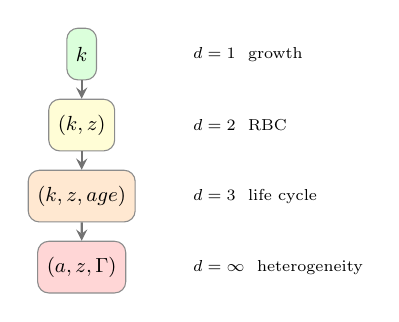
\begin{tikzpicture}[scale=0.82, transform shape,
  sbox/.style={rectangle, rounded corners, draw=black!45, align=center,
               minimum height=0.8cm, inner sep=4pt, font=\small},
  arr/.style={->, thick, >=stealth, black!55}]
  \node[sbox, fill=green!14]  (s1) at (0,0)    {$k$};
  \node[sbox, fill=yellow!16] (s2) at (0,-1.1) {$(k,z)$};
  \node[sbox, fill=orange!18] (s3) at (0,-2.2) {$(k,z,\text{age})$};
  \node[sbox, fill=red!16]    (s4) at (0,-3.3) {$(a,z,\Gamma)$};
  \draw[arr] (s1)--(s2); \draw[arr] (s2)--(s3); \draw[arr] (s3)--(s4);
  \node[font=\scriptsize, anchor=west] at (1.6,0)    {$d=1$ \ growth};
  \node[font=\scriptsize, anchor=west] at (1.6,-1.1) {$d=2$ \ RBC};
  \node[font=\scriptsize, anchor=west] at (1.6,-2.2) {$d=3$ \ life cycle};
  \node[font=\scriptsize, anchor=west] at (1.6,-3.3) {$d=\infty$ \ heterogeneity};
\end{tikzpicture}
\end{center}
\end{column}
\end{columns}
\end{frame}

%=============================================================================
\begin{frame}{The $N^{d}$ Explosion}
\begin{columns}[T]
\begin{column}{0.48\textwidth}
\small
A grid places $N$ points \emph{per dimension}, so $d$ dimensions cost $N^{d}$. With $N=100$:
\medskip
\begin{center}\footnotesize
\begin{tabularx}{\linewidth}{@{}>{\raggedright\arraybackslash}p{1.1cm} >{\raggedleft\arraybackslash}X >{\raggedright\arraybackslash}p{2.4cm}@{}}
\toprule
$d$ & \textbf{points} & \\
\midrule
$1$  & $10^{2}$  & trivial \\
$2$  & $10^{4}$  & manageable \\
$5$  & $10^{10}$ & infeasible \\
$10$ & $10^{20}$ & absurd \\
\bottomrule
\end{tabularx}
\end{center}
\medskip
\textbf{Linear in resolution, exponential in dimension.} Every extra state variable multiplies the cost by another $N$.
\end{column}
\begin{column}{0.49\textwidth}
\begin{cautionbox}[title=\textbf{And it is worse than it looks}]\small
Even at a coarse three points per axis, $d=20$ needs $3^{20}\approx3.5\times10^{9}$ points; at five points, $9.5\times10^{13}$.
\medskip
\textbf{Sparse grids delay this and do not remove it} --- 5.B3 measured exactly how much they buy.
\end{cautionbox}
\medskip
\begin{takeawaybox}\footnotesize
Note what is \emph{not} the problem: storage of the answer. The policy function is a smooth object. It is the \textbf{construction} that costs $N^{d}$, which is 7.A1's ``the bottleneck moves''.
\end{takeawaybox}
\end{column}
\end{columns}
\vspace{1mm}
\src{Ledger \texttt{param\_count.tensor\_grid\_points}. Code: \repo{tools/figures/s07_generate.py}{s07\_generate.py}, \texttt{run\_param\_count}.}
\end{frame}

%=============================================================================
\begin{frame}{What the Classical Toolkit Gives Up}
\begin{columns}[T]
\begin{column}{0.49\textwidth}
\small
Sessions 3--5 built four methods, and each bought its tractability with a concession:
\medskip
\begin{itemize}\small\setlength{\itemsep}{1.1mm}
  \item \textbf{grid VFI} --- exhaustive, and $N^{d}$;
  \item \textbf{perturbation} --- gives up global validity for speed and dimension. 5.A6 measured the cost: $1.8$ decades of accuracy at half the steady state;
  \item \textbf{Chebyshev} --- superb on smooth functions, and 5.B2 showed what a kink does to it;
  \item \textbf{finite elements} --- handles the kink, if you already know where it is.
\end{itemize}
\end{column}
\begin{column}{0.48\textwidth}
\begin{takeawaybox}[title=\textbf{The common structure}]\small
All four \textbf{choose the approximating family before looking at the solution}, and all four pay for dimension in the size of that family.
\medskip
7.A2's Theorem 6 says this is not an accident of the four we picked: \emph{any} basis fixed in advance is capped at $m^{-2/d}$.
\end{takeawaybox}
\medskip
\begin{examplebox}\footnotesize
So the opportunity is precise: replace the fixed family with a \textbf{learned} one, and replace the grid with \textbf{sampling}. That is the entire proposal, and the rest of this deck is its execution.
\end{examplebox}
\end{column}
\end{columns}
\end{frame}

%=============================================================================
\begin{frame}{What Deep Learning Actually Offers Here}
\begin{columns}[T]
\begin{column}{0.49\textwidth}
\small
\textbf{1. Approximation that scales.} A network's parameter count grows with \emph{width and depth}, not with $N^{d}$. Adding a state variable adds one input --- a row of weights, not a factor of $N$.
\medskip

\textbf{2. Differentiation for free.} 4.A4's reverse mode gives the whole gradient for about the cost of one evaluation, so a loss built from equilibrium conditions can be differentiated without anyone writing a Jacobian.
\medskip

\textbf{3. Hardware.} The arithmetic is dense matrix multiplication --- what a GPU exists to do.
\end{column}
\begin{column}{0.48\textwidth}
\begin{conceptbox}[title=\textbf{The AlphaGo reframing}]\small
Go has around $10^{170}$ states --- a state space no grid will ever cover. What worked was not a better grid but a different posture: \textbf{sample states, evaluate them with a network, and improve the network from what the samples say}.
\medskip
A macro model is the same shape of problem, with a known transition and a known reward.
\end{conceptbox}
\smallskip
{\footnotesize And one honest difference: we \emph{know} our model --- which is why this deck needs no exploration at all. S8 is what happens when you give that up.}
\end{column}
\end{columns}
\end{frame}

%=============================================================================
\begin{frame}{The Running Example}
\begin{columns}[T]
\begin{column}{0.52\textwidth}
\small
The model solved in this deck is the one 3.A4, 4.B5, 5.A6 and 5.B6 already solved --- \textbf{deliberately}, because it is the only way the comparison means anything.
\medskip

\textbf{Deterministic form, for the theory:} $u=\log c$, $\delta=1$, $f(k)=k^{\alpha}$. Then the policy is known in closed form,
\[
  k'=\alpha\beta\,k^{\alpha},
\]
which is 1.B1's benchmark: \emph{if a method cannot recover this, do not trust it on anything harder}.
\medskip

\textbf{Quarterly stochastic form, for the solve:} $\alpha=0.33$, $\beta=0.99$, $\delta=0.025$, $\log z$ an AR(1) with $\rho=0.95$, $\sigma=0.007$, discretised by Rouwenhorst to seven states.
\end{column}
\begin{column}{0.45\textwidth}
\begin{takeawaybox}[title=\textbf{Two grounds truths}]\small
The closed form checks \textbf{correctness}. The classical solutions of 4.B5 and 5.B6 check \textbf{accuracy}, because they are themselves measured.
\medskip
A method that matches the closed form and then disagrees with a validated classical solve has a bug, not a disagreement.
\end{takeawaybox}
\medskip
{\footnotesize $d=1$ deterministic, $d=2$ with the shock. \textbf{The easiest possible problem for a classical method} --- which is the point of running it.}
\end{column}
\end{columns}
\vspace{1mm}
\src{Calibration continues Session 4's, which is HW1 Q3's.}
\end{frame}

%=============================================================================
\begin{frame}{Two Roads from the Same Model}
\begin{columns}[T]
\begin{column}{0.50\textwidth}
\small
\textbf{Bellman.} Train networks to satisfy
\[
  V(k)=\max_{k'}\{u(c)+\beta V(k')\} .
\]
Two networks --- a value and a policy --- and \textbf{no first-order conditions need to be derived}. Handles kinks and discrete choices. This is 7.B2, and it has a reinforcement-learning flavour.
\medskip

\textbf{Euler.} Train one network to satisfy the first-order condition
\[
  u'(c)=\beta\,\mathbb{E}\bigl[u'(c')R'\bigr] .
\]
One network, and the FOCs must exist and be derived. Very precise where they do. \textbf{This deck.}
\end{column}
\begin{column}{0.47\textwidth}
\begin{conceptbox}[title=\textbf{Which is which, in one word}]\small
Euler-residual training is \textbf{supervised}: regress a residual against zero.
\medskip
Actor--critic is \textbf{reinforcement}: a policy gradient on the Bellman objective.
\medskip
Both are, in the end, a PyTorch optimisation --- and the loop is 3.B3's five lines.
\end{conceptbox}
\medskip
\begin{takeawaybox}\footnotesize
Neither is right in general. The Euler road is better when the FOCs are clean; the Bellman road is better when they are not --- which is most of the interesting models.
\end{takeawaybox}
\end{column}
\end{columns}
\end{frame}

%=============================================================================
\begin{frame}{The Euler Equation, and Its Residual}
\begin{columns}[T]
\begin{column}{0.55\textwidth}
\small
With $k'=g(k)$ and $c=f(k)+(1-\delta)k-g(k)$, the equilibrium satisfies
\[
  u'(c)=\beta\,u'(c')\bigl[\alpha g(k)^{\alpha-1}+1-\delta\bigr].
\tag{EE}
\]
Marginal cost of saving today equals discounted marginal benefit tomorrow.
\medskip

Define the \textbf{Euler residual} of a candidate policy $g$:
\[
  \mathcal{R}(k;g)=u'(c)-\beta u'(c')\bigl[\alpha g(k)^{\alpha-1}+1-\delta\bigr].
\]
\medskip

\textbf{The goal is to make $\mathcal{R}$ vanish} at every economically relevant $k$.
\end{column}
\begin{column}{0.42\textwidth}
\begin{takeawaybox}[title=\textbf{You have met this object}]\small
5.B1 defined exactly this and called it the residual. The projection framework was: pick a family, then make $\mathcal{R}$ small.
\medskip
\textbf{Only the family is changing.} The residual, and what ``solved'' means, are unaltered.
\end{takeawaybox}
\medskip
\begin{examplebox}\footnotesize
In practice the residual is made \textbf{unit-free} --- divided by $u'(c)$ --- so that its size reads as a consumption error, which is 3.A3's convention and the one every number in this course uses.
\end{examplebox}
\end{column}
\end{columns}
\end{frame}

%=============================================================================
\begin{frame}{Necessary, Not Sufficient}
\begin{columns}[T]
\begin{column}{0.53\textwidth}
\small
The Euler equation is \textbf{necessary}, not sufficient --- 1.B1 said so: many paths satisfy it and most explode. A complete characterisation also needs the \textbf{transversality condition} $\lim_{t}\beta^{t}u'(c_t)k_{t+1}=0$ and \textbf{feasibility}, $c\ge0$, $k'\ge0$.
\smallskip

Where a constraint binds, Kuhn--Tucker gives \textbf{three} conditions at once --- $a\ge0$, $b\ge0$, $ab=0$. The \textbf{Fischer--Burmeister} function
\[
  \varphi(a,b)=a+b-\sqrt{a^{2}+b^{2}}
\]
is zero \emph{exactly} when all three hold, so \textbf{one smooth equation replaces the complementarity}. It drops straight into the residual, and \texttt{autograd} differentiates it like anything else.
\end{column}
\begin{column}{0.44\textwidth}
\begin{cautionbox}[title=\textbf{Why this matters here}]\footnotesize
A network minimising $\mathcal{R}^{2}$ will happily find an explosive path if that makes the residual small: \textbf{the transversality condition is not in the loss}, and nothing in training imposes it. Here the bounded parameterisation does the work --- the policy is confined to a compact capital interval, so an explosive path is not representable.
\end{cautionbox}
\smallskip
{\footnotesize Here $a$ is the multiplier on $k'\ge0$ and $b$ the slack. 2.A1 met $\varphi$ as a \textbf{penalty}, $\lambda\sum\varphi(\cdot)^{2}$ --- ``how a neural solver enforces what it cannot impose''. This is the other half of that sentence.}
\end{column}
\end{columns}
\vspace{1mm}
\src{Fischer \& Burmeister (1992). The function is non-smooth only at the origin, which is where both conditions bind exactly.}
\end{frame}

%=============================================================================
\begin{frame}{From Residual to Loss}
\begin{columns}[T]
\begin{column}{0.55\textwidth}
\small
Three steps and the method is complete.
\smallskip
\textbf{1.} Approximate the policy by a network, $g(k)\approx\mathcal{N}(k;\theta)$.
\smallskip
\textbf{2.} Sample states $k_i\sim D(k)$ --- uniform on a band, or ergodic.
\smallskip
\textbf{3.} Minimise the mean squared residual
\[
  \mathcal{L}(\theta)=\mathbb{E}_{k\sim D}\bigl[\mathcal{R}(k;\mathcal{N}_\theta)^{2}\bigr]
  \;\approx\;\frac{1}{N}\sum_{i=1}^{N}\mathcal{R}(k_i;\mathcal{N}_\theta)^{2},
\]
with every derivative taken by \texttt{autograd}.
\end{column}
\begin{column}{0.42\textwidth}
\begin{takeawaybox}[title=\textbf{It is supervised learning}]\small
The ``label'' on every sampled state is \textbf{zero}. So 7.A3 applies unchanged --- mini-batches, Adam, a schedule --- with one difference worth savouring: \textbf{the labels are not noisy, and the training set is unlimited.}
\end{takeawaybox}
\smallskip
{\footnotesize The intuition is a mean-value one: a policy satisfying the Euler equation \emph{on average} over the region that matters is close to the equilibrium policy, and a large average residual means optimality is violated somewhere.}
\end{column}
\end{columns}
\end{frame}

%=============================================================================
\begin{frame}{This Is 5.B5, with One Substitution}
\begin{columns}[T]
\begin{column}{0.55\textwidth}
\small
Write the loss as the integral it is:
\[
  \mathcal{L}(\theta)=\mathbb{E}_{k\sim D}\bigl[\mathcal{R}(k)^{2}\bigr]
  =\int \mathcal{R}(k)^{2}\,D(k)\,\mathrm{d}k ,
\]
and compare 5.B5's weighted residual method, which chose $\theta$ to minimise
\[
  \int w(k)\,\mathcal{R}(k)^{2}\,\mathrm{d}k .
\]
They are the \textbf{same object}, with $w(k)=D(k)$: \textbf{the sampling distribution is the weight function.}
\end{column}
\begin{column}{0.42\textwidth}
\begin{takeawaybox}[title=\textbf{The promise 5.B1 made}]\small
``Replace $\sum\theta_i\psi_i$ by $\mathcal{N}(x;\theta)$ and the framework is unchanged. That is S7.''
\medskip
Here it is, discharged: \textbf{a neural Euler solver is least-squares projection on a learned basis, with the weight function chosen by where you sample.}
\end{takeawaybox}
\smallskip
{\footnotesize Read it both ways: $D$ uniform on a grid $\approx$ \textbf{collocation} with equal weights; $D$ the stationary distribution buys accuracy \textbf{where the model spends its time}.}
\end{column}
\end{columns}
\vspace{1mm}
\src{Fern\'andez-Villaverde \& Guerr\'on-Quintana, \emph{Solution Methods} IV. This is the frame 5.B1 promised.}
\end{frame}

%=============================================================================
\begin{frame}{What Is Genuinely Different from Collocation}
\begin{columns}[T]
\begin{column}{0.49\textwidth}
\small
\textbf{Collocation and Galerkin} require two choices made in advance: a \textbf{basis} $\{\psi_i\}$, and a set of \textbf{collocation points} or weight functions. The residual is then driven to zero at those points, or made orthogonal to those functions.
\medskip

\textbf{The network approach} makes neither choice. There is no basis to select, and no node set: the residual is averaged over \textbf{sampled} states, so the weighting is implicit in the sampler.
\end{column}
\begin{column}{0.48\textwidth}
\begin{center}\footnotesize
\begin{tabularx}{\linewidth}{@{}>{\raggedright\arraybackslash}p{1.5cm} >{\raggedright\arraybackslash}X >{\raggedright\arraybackslash}X@{}}
\toprule
& \textbf{projection} & \textbf{network} \\
\midrule
family & chosen & learned \\
where & nodes & samples \\
weight & $w(\cdot)$, chosen & $D(\cdot)$, sampled \\
solve & root-find on $\theta$ & descent on $\theta$ \\
scaling & $m^{-2/d}$ & see 7.A2 \\
\bottomrule
\end{tabularx}
\end{center}
\medskip
\begin{cautionbox}\footnotesize
The last row is the whole bet, and 7.A2 was careful about it: the escape from $m^{-2/d}$ is real \textbf{and} conditional on the function being one a few ridge directions can express.
\end{cautionbox}
\end{column}
\end{columns}
\end{frame}

%=============================================================================
\begin{frame}{The Stochastic Case: an Expectation Inside the Residual}
\begin{columns}[T]
\begin{column}{0.55\textwidth}
\small
With a productivity shock the Euler equation carries a conditional expectation:
\[
  u'(c_t)=\beta\,\mathbb{E}_{z'\mid z}\!\bigl[u'(c_{t+1})\bigl(\alpha k_{t+1}^{\alpha-1}z'+1-\delta\bigr)\bigr].
\]
There is no closed form for it, so it has to be computed --- inside the loss, at every step.
\medskip

The blunt option is Monte Carlo over $J$ draws:
\[
  \widehat{\mathcal{R}}(k_i)=u'(c_i)-\frac{\beta}{J}\sum_{j=1}^{J}u'(c'_{ij})R'_{ij} .
\]
\end{column}
\begin{column}{0.42\textwidth}
\begin{cautionbox}[title=\textbf{Two layers of sampling}]\small
An \textbf{outer} average over states $k_i\sim D$ --- that is the loss --- and an \textbf{inner} average over shocks $z'$ --- that is the expectation.
\medskip
Different things, different remedies. Outer noise makes descent stochastic and is \emph{useful}; \textbf{inner noise contaminates the residual itself}.
\end{cautionbox}
\smallskip
{\footnotesize Monte Carlo error falls like $1/\sqrt J$, and that noise enters \emph{every} gradient. 4.B2 had a better instrument.}
\end{column}
\end{columns}
\end{frame}

%=============================================================================
\begin{frame}{Gauss--Hermite, and Why the Loss Stays Differentiable}
\begin{columns}[T]
\begin{column}{0.55\textwidth}
\small
\textbf{1. The problem.} A Monte-Carlo estimate puts noise \emph{inside} the residual. Unlike 7.A3's outer sampling noise, which averages out and even helps, \textbf{inner noise corrupts the very quantity being driven to zero}.
\smallskip

\textbf{2. The fix.} 4.B2's quadrature: $J$ \textbf{deterministic} nodes and weights,
\[
  \mathbb{E}_{z'\mid z}[h(z')]\approx\sum_{j=1}^{J}w_j\,h(z'_j),
\]
exact whenever $h$ is a polynomial of degree $\le 2J-1$ against the Gaussian weight. Smooth integrands are nearly polynomial, so \textbf{five to seven nodes match thousands of draws}.
\end{column}
\begin{column}{0.42\textwidth}
\begin{takeawaybox}[title=\textbf{3. Why it is safe for \texttt{autograd}}]\footnotesize
The nodes and weights are \textbf{constants}, so the loss is a fixed weighted sum of smooth network outputs and the tape differentiates straight through. Mini-batching changes only \emph{which} states enter the sum. And we sample \textbf{exogenous} shocks, never policy-dependent randomness --- so no reparameterisation trick is needed.
\medskip
\textbf{4. And in this deck.} The shock is a \textbf{seven-state Rouwenhorst chain}, so the expectation is an \emph{exact finite sum} and none of this arises. \textbf{Gauss--Hermite is what you reach for when the shock is continuous.}
\end{takeawaybox}
\end{column}
\end{columns}
\vspace{1mm}
\src{For a log-normal shock, change variables to a standard normal and read the nodes off the table.}
\end{frame}

%=============================================================================
\begin{frame}{The Policy Network, and Feasibility by Construction}
\begin{columns}[T]
\begin{column}{0.52\textwidth}
\small
The architecture is unremarkable --- a small MLP with a sigmoid on the output, $\sigma_1$ a ReLU or $\tanh$:
\[
  \mathcal{N}(k;\theta)=\sigma_2\bigl(W_2\,\sigma_1(W_1k+b_1)+b_2\bigr).
\]
What matters is what is done with it. The sigmoid gives $s\in(0,1)$, so set
\[
  g(k)=s\cdot\bigl[f(k)+(1-\delta)k-\varepsilon\bigr],
\]
so that $0\le g(k)\le f(k)+(1-\delta)k$ \textbf{identically}.
\end{column}
\begin{column}{0.45\textwidth}
\begin{takeawaybox}[title=\textbf{Why this is not a detail}]\small
$u'(c)=c^{-\sigma}$ \textbf{diverges} as $c\to0$: one infeasible sample gives an enormous residual, an enormous gradient, and a destroyed network.
\medskip
The bound is in the \textbf{parameterisation}, not bolted on afterwards, so an infeasible policy is not representable. The $\varepsilon$ keeps marginal utility finite at the edge.
\end{takeawaybox}
\medskip
{\footnotesize \textbf{Alternatives:} softplus (positive, smooth, unbounded above); hard \texttt{clamp} (simple, and \emph{kills the gradient} at the boundary); log-parameterisation.}
\end{column}
\end{columns}
\vspace{1mm}
\src{\textbf{This is 7.B3's theme in miniature}: a property imposed by architecture rather than hoped for.}
\end{frame}

%=============================================================================
\begin{frame}[fragile]{The Training Loop}
\begin{columns}[T]
\begin{column}{0.53\textwidth}
\small
\begin{lstlisting}
for it in range(iters):
    opt.zero_grad()               # 1 ZERO
    k  = sample_states(batch)     # 2 FORWARD
    c  = cash(k) * net(k)         #   feasible
    kp = cash(k) - c
    rhs = 0.0
    for j in range(n_z):          #   exact sum
        cp = cash(kp, j) * net(kp, j)
        rhs += Pi[:, j] * R(kp, j) / cp
    resid = 1.0 - c * beta * rhs
    loss = (resid**2).mean()      # 3 SCORE
    loss.backward()               # 4 BACKWARD
    opt.step()                    # 5 STEP
\end{lstlisting}
\end{column}
\begin{column}{0.44\textwidth}
\begin{takeawaybox}[title=\textbf{Recognise it}]\small
The five numbered comments are 3.B3's loop, \textbf{zero, forward, score, backward, step}, in that order and unchanged. \textbf{Everything else --- the four lines that build \texttt{resid} --- is the Euler equation.}
\end{takeawaybox}
\medskip
\begin{examplebox}\footnotesize
The network is called \textbf{twice} --- at $k$ and at $k'$ --- so the graph holds the policy composed with itself and the gradient flows through both. This is not a regression on a fixed target.
\medskip
\textbf{Pros:} one network, precise, grounded. \textbf{Cons:} no value function, and the FOCs must exist.
\end{examplebox}
\end{column}
\end{columns}
\vspace{1mm}
\src{Full code in \repo{labs/L07_ML_and_Deep_Growth.ipynb}{L07}, Parts 4--5.}
\end{frame}

%=============================================================================
\begin{frame}{Where to Sample: the Choice That Is Easy to Miss}
\begin{columns}[T]
\begin{column}{0.52\textwidth}
\small
$D(k)$ is a \textbf{modelling decision}, not a technicality, because it is the weight function.
\medskip

\textbf{Uniform over a band.} Simple, and it spends equal effort everywhere --- including regions the economy visits with probability near zero. Accuracy is spread thin.
\medskip

\textbf{The ergodic distribution.} Simulate the model under the current policy and train where it actually goes. Accuracy concentrates where it matters, and the objective is the economically meaningful one.
\end{column}
\begin{column}{0.45\textwidth}
\begin{cautionbox}[title=\textbf{And the trap}]\small
The ergodic distribution depends on the policy, which is what is being learned. Train only where the \emph{current} policy goes and it can settle into a small region, satisfy the Euler equation beautifully there, and be \textbf{arbitrarily wrong outside it} --- with a small loss reporting success.
\end{cautionbox}
\smallskip
{\footnotesize The practical answer is a \textbf{mixture} --- mostly ergodic, part from a wider band. And always \textbf{evaluate somewhere other than where you trained} (7.B3).}
\end{column}
\end{columns}
\vspace{1mm}
\src{The worked example below samples \textbf{uniformly} on $[0.5k^{*},1.5k^{*}]$, which is 5.B6's band exactly.}
\end{frame}

%=============================================================================
\begin{frame}{The Same Model, a Fifth Way}
\begin{columns}[T]
\begin{column}{0.52\textwidth}
\small
Everything above, applied to the quarterly RBC model of 5.B6 --- the \textbf{same} \texttt{Proj} object, chain, band $[0.5k^{*},1.5k^{*}]$ and unit-free metric. Nothing is re-specified.
\smallskip
\begin{itemize}\small\setlength{\itemsep}{1mm}
  \item \textbf{Network:} 3 hidden layers of 64, tanh; c = sigmoid(net)*cash, $8{,}961$ parameters.
  \item \textbf{States:} $1{,}024$ fresh uniform draws per step; \textbf{nothing is reused}.
  \item \textbf{Expectation:} exact over the seven states.
  \item \textbf{Optimizer:} Adam, lr 3e-3 cosine-decayed to 1e-5, $30{,}000$ steps.
\end{itemize}
\end{column}
\begin{column}{0.45\textwidth}
\begin{conceptbox}[title=\textbf{What is being tested}]\small
The \textbf{easiest} problem in the course for a classical method --- one endogenous state, a smooth policy, a known band --- and therefore the hardest case for the network. Running it here rather than on something flattering is the point.
\end{conceptbox}
\smallskip
\begin{cautionbox}\footnotesize
\textbf{Trained to a plateau, not a budget.} The last tenth of training improved the loss by only 34\%; a five-fold rise in parameters and iterations moved the headline number by $0.02$ of a decade.
\end{cautionbox}
\end{column}
\end{columns}
\vspace{1mm}
\src{Ledger \texttt{worked\_nn\_growth}. The generator \emph{imports} \texttt{tools/figures/s05\_generate.py}, so 7.B1 and 5.B6 solve the same model by construction. Run on a compute node, CPU, float64. Code: \repo{tools/figures/s07_generate.py}{s07\_generate.py}, \texttt{run\_worked\_nn\_growth}; \repo{labs/L07_ML_and_Deep_Growth.ipynb}{L07} Part 5.}
\end{frame}

%=============================================================================
\begin{frame}{Did It Converge?}
\begin{columns}[T]
\begin{column}{0.52\textwidth}
\begin{center}
\begin{tikzpicture}
\begin{axis}[
    width=7.6cm, height=4.4cm,
    xlabel={\scriptsize iteration}, ylabel={\scriptsize $\log_{10}$ mean squared residual},
    tick label style={font=\scriptsize}, label style={font=\scriptsize},
    axis x line*=bottom, axis y line*=left,
    scaled x ticks=false, /pgf/number format/1000 sep={},
    xmin=0, xmax=31000]
  \addplot[very thick, RedTitle] coordinates {(1000.0000,-4.8633) (2000.0000,-4.9158) (3000.0000,-5.1222) (4000.0000,-5.2354) (5000.0000,-5.5166) (6000.0000,-5.4355) (7000.0000,-5.4392) (8000.0000,-5.6220) (9000.0000,-5.5472) (10000.0000,-5.4905) (11000.0000,-5.6342) (12000.0000,-5.6243) (13000.0000,-5.3578) (14000.0000,-5.6973) (15000.0000,-5.6940) (16000.0000,-6.0350) (17000.0000,-5.7459) (18000.0000,-5.5277) (19000.0000,-5.8154) (20000.0000,-5.6924) (21000.0000,-5.3419) (22000.0000,-6.0123) (23000.0000,-5.9922) (24000.0000,-5.8575) (25000.0000,-5.8544) (26000.0000,-5.9796) (27000.0000,-5.8153) (28000.0000,-6.1060) (29000.0000,-5.9278) (30000.0000,-5.9973)};
\end{axis}
\end{tikzpicture}
\end{center}
\end{column}
\begin{column}{0.45\textwidth}
\small
The loss falls by about four decades and then \textbf{flattens, noisily}. The noise is the outer sampling --- a fresh batch of states every step --- and it never disappears, because the loss is an expectation being estimated, not a fixed number being minimised.
\medskip

\begin{cautionbox}\footnotesize
\textbf{This curve cannot tell you the answer is right.} It is the training loss, measured on the states the optimizer just used. 7.A3's warning applies with full force, and the only honest verdict comes from evaluating somewhere else.
\end{cautionbox}
\end{column}
\end{columns}
\vspace{1mm}
\src{``One decade'' is a factor of ten in the error (3.A1). Ledger \texttt{fig\_nn\_loss}, recorded every $1{,}000$ iterations. Code: \repo{tools/figures/s07_generate.py}{s07\_generate.py}.}
\end{frame}

%=============================================================================
\begin{frame}{The Policy It Learned}
\begin{columns}[T]
\begin{column}{0.54\textwidth}
\begin{center}
\begin{tikzpicture}
\begin{axis}[
    width=8.0cm, height=4.4cm,
    xlabel={\scriptsize capital $k$}, ylabel={\scriptsize $k'-k$},
    tick label style={font=\scriptsize}, label style={font=\scriptsize},
    axis x line*=bottom, axis y line*=left,
    xmin=14, xmax=43]
  \addplot[very thick, RedTitle] coordinates {(14.1742,-1.1975) (14.4591,-1.1113) (14.7440,-1.1030) (15.0289,-1.0765) (15.3138,-1.0434) (15.5988,-1.0116) (15.8837,-0.9818) (16.1686,-0.9534) (16.4535,-0.9256) (16.7384,-0.8982) (17.0233,-0.8710) (17.3082,-0.8440) (17.5931,-0.8171) (17.8780,-0.7905) (18.1629,-0.7641) (18.4478,-0.7380) (18.7327,-0.7123) (19.0177,-0.6869) (19.3026,-0.6619) (19.5875,-0.6371) (19.8724,-0.6127) (20.1573,-0.5886) (20.4422,-0.5647) (20.7271,-0.5410) (21.0120,-0.5175) (21.2969,-0.4941) (21.5818,-0.4709) (21.8667,-0.4478) (22.1517,-0.4247) (22.4366,-0.4017) (22.7215,-0.3787) (23.0064,-0.3559) (23.2913,-0.3331) (23.5762,-0.3104) (23.8611,-0.2878) (24.1460,-0.2654) (24.4309,-0.2432) (24.7158,-0.2212) (25.0007,-0.1995) (25.2857,-0.1781) (25.5706,-0.1570) (25.8555,-0.1363) (26.1404,-0.1159) (26.4253,-0.0960) (26.7102,-0.0765) (26.9951,-0.0574) (27.2800,-0.0388) (27.5649,-0.0206) (27.8498,-0.0029) (28.1347,0.0144) (28.4196,0.0313) (28.7046,0.0478) (28.9895,0.0638) (29.2744,0.0794) (29.5593,0.0947) (29.8442,0.1096) (30.1291,0.1241) (30.4140,0.1384) (30.6989,0.1523) (30.9838,0.1659) (31.2687,0.1793) (31.5536,0.1924) (31.8386,0.2053) (32.1235,0.2179) (32.4084,0.2304) (32.6933,0.2426) (32.9782,0.2547) (33.2631,0.2666) (33.5480,0.2783) (33.8329,0.2899) (34.1178,0.3013) (34.4027,0.3127) (34.6876,0.3239) (34.9725,0.3350) (35.2575,0.3460) (35.5424,0.3569) (35.8273,0.3677) (36.1122,0.3784) (36.3971,0.3891) (36.6820,0.3996) (36.9669,0.4101) (37.2518,0.4206) (37.5367,0.4310) (37.8216,0.4413) (38.1065,0.4516) (38.3915,0.4619) (38.6764,0.4722) (38.9613,0.4824) (39.2462,0.4926) (39.5311,0.5028) (39.8160,0.5130) (40.1009,0.5233) (40.3858,0.5336) (40.6707,0.5439) (40.9556,0.5544) (41.2405,0.5649) (41.5254,0.5755) (41.8104,0.5862) (42.0953,0.5970) (42.3802,0.6080)};
  \addplot[gray!60, dashed, thick, domain=14:43, samples=2] {0};
  \draw[gray!70, dotted, thick] (axis cs:28.348,-1.2) -- (axis cs:28.348,1.2);
  \node[font=\tiny, anchor=south west, gray!50!black] at (axis cs:28.348,0.55) {$k^{*}$};
\end{axis}
\end{tikzpicture}
\end{center}
\end{column}
\begin{column}{0.43\textwidth}
\small
Plotted as \textbf{net saving} $k'-k$ at the middle shock state, because the level $k'$ against $k$ is visually a $45^{\circ}$ line for every method and shows nothing.
\medskip

The shape is right: saving positive below $k^{*}$, negative above, and the \textbf{zero crossing at $k^{*}$}. The curve is smooth --- no staircase, because there is no grid.
\medskip
\begin{takeawaybox}\footnotesize
Compare 4.B5, whose grid search quantised saving into two values across $36$ states. That artefact is simply gone. \textbf{Smoothness is a genuine and free gain here.}
\end{takeawaybox}
\end{column}
\end{columns}
\vspace{1mm}
\src{Ledger \texttt{fig\_nn\_saving}, middle shock state. Deviation, not level, per the house rule. Code: \repo{tools/figures/s07_generate.py}{s07\_generate.py}.}
\end{frame}

%=============================================================================
\begin{frame}{Where the Error Actually Lives}
\begin{columns}[T]
\begin{column}{0.54\textwidth}
\begin{center}
\begin{tikzpicture}
\begin{axis}[
    width=8.0cm, height=4.4cm,
    xlabel={\scriptsize capital $k$}, ylabel={\scriptsize $\log_{10}$ max Euler error},
    tick label style={font=\scriptsize}, label style={font=\scriptsize},
    axis x line*=bottom, axis y line*=left,
    xmin=14, xmax=43, ymin=-4.2, ymax=-1.2]
  \addplot[very thick, RedTitle] coordinates {(14.1742,-1.5754) (14.6507,-2.4677) (15.1271,-2.1965) (15.6035,-2.5340) (16.0800,-2.8160) (16.5564,-3.2187) (17.0329,-3.2032) (17.5093,-3.5290) (17.9858,-3.4385) (18.4622,-3.3817) (18.9386,-3.3895) (19.4151,-3.4401) (19.8915,-3.5333) (20.3680,-3.6716) (20.8444,-3.5950) (21.3209,-3.5883) (21.7973,-3.5350) (22.2738,-3.5200) (22.7502,-3.5407) (23.2266,-3.5091) (23.7031,-3.3815) (24.1795,-3.3012) (24.6560,-3.2584) (25.1324,-3.2453) (25.6089,-3.2571) (26.0853,-3.2909) (26.5618,-3.3455) (27.0382,-3.4210) (27.5146,-3.5191) (27.9911,-3.6445) (28.4675,-3.5959) (28.9440,-3.5419) (29.4204,-3.5002) (29.8969,-3.4702) (30.3733,-3.4518) (30.8498,-3.4198) (31.3262,-3.3689) (31.8026,-3.3428) (32.2791,-3.3456) (32.7555,-3.3840) (33.2320,-3.4638) (33.7084,-3.4759) (34.1849,-3.4943) (34.6613,-3.4526) (35.1377,-3.5018) (35.6142,-3.5618) (36.0906,-3.5370) (36.5671,-3.5172) (37.0435,-3.3417) (37.5200,-3.2835) (37.9964,-3.3316) (38.4729,-3.4945) (38.9493,-3.5654) (39.4257,-3.5898) (39.9022,-3.7054) (40.3786,-3.5602) (40.8551,-3.4139) (41.3315,-3.1743) (41.8080,-2.9687) (42.2844,-2.2198)};
  \draw[gray!70, dotted, thick] (axis cs:28.348,-4.2) -- (axis cs:28.348,-1.2);
  \node[font=\tiny, anchor=west, gray!50!black] at (axis cs:28.348,-1.45) {$k^{*}$};
\end{axis}
\end{tikzpicture}
\end{center}
\end{column}
\begin{column}{0.43\textwidth}
\small
\begin{center}\footnotesize
\begin{tabularx}{\linewidth}{@{}>{\raggedright\arraybackslash}X >{\raggedleft\arraybackslash}p{2.0cm}@{}}
\toprule
\textbf{Where} & \textbf{$\log_{10}$ err} \\
\midrule
at $0.5k^{*}$ (the edge) & $-1.58$ \\
at $k^{*}$ & $\mathbf{-3.63}$ \\
at $1.5k^{*}$ (the edge) & $-1.96$ \\
\bottomrule
\end{tabularx}
\end{center}
\medskip
\begin{takeawaybox}\footnotesize
\textbf{Two decades --- a factor of a hundred --- separate the middle of the band from its edges}, and the single worst point is at $k=14.17$ --- \textbf{exactly the lower boundary}.
\medskip
Drop the outer $5\%$ at each end and the maximum improves from $-1.61$ to $-2.54$.
\end{takeawaybox}
\end{column}
\end{columns}
\vspace{1mm}
\src{Ledger \texttt{worked\_nn\_growth}, \texttt{fig\_nn\_errk}. \textbf{The lesson generalises:} a sampled method is weakest at the edge of the region it sampled, so \emph{sample wider than you intend to evaluate}. Code: \repo{tools/figures/s07_generate.py}{s07\_generate.py}; \repo{labs/L07_ML_and_Deep_Growth.ipynb}{L07} Part 5.}
\end{frame}

%=============================================================================
\begin{frame}{One Model, Five Methods}
\vspace{-1mm}
\begin{center}\footnotesize
\begin{tabularx}{\linewidth}{@{}>{\raggedright\arraybackslash}X >{\raggedleft\arraybackslash}p{2.0cm} >{\raggedleft\arraybackslash}p{1.9cm} >{\raggedleft\arraybackslash}p{2.1cm} >{\raggedleft\arraybackslash}p{2.1cm}@{}}
\toprule
\textbf{Method} & \textbf{numbers stored} & \textbf{seconds} & \textbf{$\max$ err, band} & \textbf{$\max$ err, near $k^{*}$} \\
\midrule
global VFI (4.B5) & $2{,}100$ & $0.941$ & $-2.51$ & $-2.82$ \\
perturbation{,} 1st order & $4$ & $0.000$ & $-2.56$ & $-4.01$ \\
perturbation{,} 2nd order & $12$ & $0.020$ & $-4.50$ & $-6.14$ \\
Chebyshev collocation & $56$ & $0.133$ & $-6.40$ & $-6.82$ \\
neural network (7.B1) & $8{,}961$ & $343.257$ & $-1.61$ & $-3.25$ \\
\bottomrule
\end{tabularx}
\end{center}
\medskip
\begin{columns}[T]
\begin{column}{0.49\textwidth}
\begin{takeawaybox}\footnotesize
\textbf{Chebyshev wins on every axis at once}: $56$ numbers, a tenth of a second, and five decades better than the network across the band. On this problem it is not close.
\end{takeawaybox}
\end{column}
\begin{column}{0.49\textwidth}
\begin{cautionbox}\footnotesize
The first four rows are \textbf{read from the Session 5 ledger}, not recomputed, so the comparison cannot drift as either side is edited.
\end{cautionbox}
\end{column}
\end{columns}
\vspace{1mm}
\src{Ledger \texttt{five\_methods}; rows 1--4 from \texttt{s05\_numbers.json} key \texttt{three\_methods}. Errors are $\log_{10}$ of the maximum unit-free Euler residual over $2{,}000$ off-grid states. Code: \repo{tools/figures/s07_generate.py}{s07\_generate.py}, \repo{tools/figures/s05_generate.py}{s05\_generate.py}.}
\end{frame}

%=============================================================================
\begin{frame}{Read That Table Before You Believe the Hype}
\begin{columns}[T]
\begin{column}{0.53\textwidth}
\small
\textbf{The network came last, and it deserved to.} It stored $8{,}961$ numbers against Chebyshev's $56$, took $2581$ times as long, and was about \textbf{five decades} less accurate across the band.
\medskip

This is not a failure of the implementation. \textbf{It is exactly what 7.A2 predicted:} on a smooth, low-dimensional function a spectral basis is close to optimal, and an adaptive basis has nothing to adapt to. The same table appeared there with $\sin$ and $e^{-x}\sin 3x$ in place of a policy function.
\end{column}
\begin{column}{0.44\textwidth}
\begin{takeawaybox}[title=\textbf{So why learn the method?}]\small
Because \textbf{every column of that table scales differently.}
\medskip
Chebyshev's $56$ coefficients become $56^{d}$ --- or a Smolyak set that still grows. The network's $8{,}961$ parameters become $8{,}961$ plus one row of weights per added state.
\medskip
\textbf{The crossover is not at $d=1$. It is out where the classical methods stop running at all.}
\end{takeawaybox}
\end{column}
\end{columns}
\vspace{1mm}
\src{And the honest corollary: \textbf{if a classical method can solve your model, use it.} The network is for the models where none can.}
\end{frame}

%=============================================================================
\begin{frame}{Takeaways, and What 7.B2 Changes}
\begin{columns}[T]
\begin{column}{0.55\textwidth}
\begin{takeawaybox}\small
\begin{itemize}\small\setlength{\itemsep}{1.1mm}
  \item An economic model supplies its own training target: the \textbf{label on every sampled state is zero}, and the sample is unlimited.
  \item The loss $\int\mathcal{R}^{2}D(k)\,\mathrm{d}k$ \textbf{is} 5.B5's least-squares weighted residual, with $w=D$. \textbf{The sampling distribution is the weight function.}
  \item Feasibility belongs in the \textbf{parameterisation}, not in a clip: $c=\sigma(\cdot)\times$ cash.
  \item Measured: the network is \textbf{last of five} on this model, and its error is worst \textbf{at the edge of the sampled band} --- two decades worse than at $k^{*}$.
\end{itemize}
\end{takeawaybox}
\end{column}
\begin{column}{0.42\textwidth}
\begin{conceptbox}[title=\textbf{Bridge to 7.B2}]\small
This deck needed the \textbf{first-order conditions}. Many models do not have usable ones --- kinks, discrete choices, occasionally binding constraints.
\medskip
\textbf{7.B2} goes back to the Bellman equation instead and trains \emph{two} networks, a value and a policy, against each other. No FOCs required --- and a new problem in their place.
\end{conceptbox}
\end{column}
\end{columns}
\end{frame}

\end{document}
